\section{Additional Reproducibility Details}
\label{app:repro}

\paragraph{Dataset.} Scaled WorldConsistMem is generated with seed 100. Smoke validation confirms gold Acc $=$ BCR $=$ ConsAcc $=$ 1 and Acc--$\Phi$ separation under controlled corruptions.

\paragraph{Readers.} Symbolic exact-match scoring is used for the full scaled study. The LLM condition uses \texttt{Qwen2.5-3B-Instruct-4bit} with frozen short-form JSON decoding (temperature 0; max tokens 48) on the H4 subset (18 worlds / 192 bundles / 1{,}260 queries).

\paragraph{Systems.} Headline reference systems: B1 capacity-limited compact flat; B3 recency retrieval; B4 BM25 retrieval; H0 structured hierarchical reference. Ablations and capacity sweeps are reported in the released artefacts.

\paragraph{Metrics.} Primary consistency rate: BCR. Complementary: CSR, ConsAcc / PConsAcc grid, $\Gapq$, family violation rates. World-level bootstrap 95\% CIs accompany BCR/CSR (and world-mean Acc) in frozen CSVs.

\paragraph{Labelled rescue sanity (not Option A).} Re-evaluating gold answers on the H4 subset yields Acc$=$BCR$=$ConsAcc$=$1 with zero violations. Additional labelled robustness (seeds 100--105; relation density; distractors; shortcut baselines) is reported in Section~\ref{sec:robustness} and Tables~\ref{tab:shortcuts}--\ref{tab:density}; these artefacts are not merged into Option~A tables. Stronger LLM readers were not completed in this environment.

\section{Artifact Checklist}
\label{app:artifacts}

Released artefacts accompanying this submission include: dataset generators and manifests; symbolic system results and predictions; Qwen H4 system/query-family/constraint-family results; partial-consistency recomputes; corruption-suite metrics; and figure sources corresponding to Figures~\ref{fig:pipeline}--\ref{fig:constraints}. Anonymized supplementary material is provided with the OpenReview submission; identifying repository URLs are omitted from this PDF.

\section{Extended Related Work}
\label{app:related}
\label{app:closest}

\subsection{Long-term memory evaluation}

LongMemEval evaluates chat assistants on long-term interactive memory through five ability axes---information extraction, multi-session reasoning, temporal reasoning, knowledge updates, and abstention---with answer accuracy as the primary metric under long-history and long-context protocols~\citep{wu2025longMemEval}. LongMemEval-V2 extends the agenda toward ``experienced colleague'' competence, adding dynamic state tracking, workflows, and premise awareness, again with per-question accuracy (and latency-oriented reporting) as the headline outcomes~\citep{wu2026longMemEvalV2}. MemoryAgentBench evaluates agent memory via incremental multi-turn interactions across competencies such as accurate retrieval, test-time learning, long-range understanding, and selective forgetting / FactConsolidation after edits, scored primarily by task or answer accuracy~\citep{hu2025memoryAgentBench}. EverMemBench targets long-horizon collaborative, multi-party dialogues and reports fine-grained recall, memory awareness, and profile understanding under QA accuracy protocols~\citep{hu2026everMemBench}. EvoMemBench organizes agent memory from a self-evolving perspective with a scope$\times$content taxonomy and reports task success or accuracy (and efficiency) across methods compared with long-context baselines~\citep{wang2026evoMemBench}. Taken together, this line provides mature protocols for long-horizon Acc and ability factorization; the measurement gap we target is joint coherence of dependent answers, not another Acc axis.

These benchmarks primarily evaluate individual query or task outcomes. WorldConsistMem does not replace ability Acc suites. It additionally evaluates whether answers within a dependent bundle jointly satisfy constraints derived from one world history. The evaluation unit is the interdependent answer set $\hat Y_b$ under $\Phi(\hat Y_b;\mathcal{C}_b)$, not a single graded QA item.

\subsection{Dynamic and evolving knowledge}

Evolving worlds are not novel by themselves. DynamicMem constructs long-horizon personal memory in real-world settings and evaluates temporal checkpoint reconstruction and related state-tracking accuracy for evolving user attributes, habits, and preferences~\citep{xie2026dynamicMem}. WorldMemArena evaluates multimodal agent memory through action--world interaction, diagnosing write, maintain, retrieve, and use stages under lifelong evolution and agentic execution protocols~\citep{liu2026worldMemArena}.

It is important to distinguish three notions that are easy to conflate. \emph{Tracking changing state} asks whether the system recovers the correct value at a time or checkpoint. \emph{Profile or lifecycle consistency} asks whether personal attributes, stage metrics, or write/use pipelines remain coherent for a user or agent trajectory. \emph{Cross-query world-history consistency} asks whether interdependent answers about current state, historical state, transitions, relations, and provenance jointly satisfy constraints induced by one shared multi-entity gold history.

\subsection{Conflict, temporal validity, and provenance}

MemConflict evaluates long-term memory systems under dynamic, static, and conditional memory conflicts, combining black-box answer correctness with white-box retrieval and ranking diagnostics, and showing that answer correctness can diverge from retrieval fitness~\citep{tao2026memConflict}. These lines diagnose conflict handling, version validity, and temporal updates at the query, retrieval, or competency level. The WorldConsistMem contrast is evaluation grain and joint structure rather than denial of those pathologies: a conflict- or update-correct single answer can still participate in an inconsistent bundle.

\subsection{Cross-query logical consistency}

\citet{salla2026crossQueryContradictions} study case-file logical consistency across interdependent queries and introduce set-level metrics including Case Satisfiability and SetConsRate. \citet{chaudhry2026logicVault} maintain persistent symbolic belief states verified with SMT-style checking and release LogicBench-Cross. Machine-checkable constraint evaluation over multi-query answer sets is therefore not universally new. WorldConsistMem's residual is application domain and constraint origin: persistent memory systems over evolving multi-entity worlds with world-history-derived constraints.

\begin{table}[t]
\centering
\caption{Closest related benchmarks and adjacent consistency work. Cells use Y / P / N for whether the feature is a \emph{primary} evaluation object as operationalized in WorldConsistMem.}
\label{tab:closest}
\scriptsize
\resizebox{\textwidth}{!}{%
\begin{tabular}{lcccccccccc}
\toprule
Work & LTM & Evol. & Bundles & Gold hist. & Trans. & Prov. & CQ constr. & Strict BCR & Partial CSR & Primary metric \\
\midrule
LongMemEval & Y & P & N & P & P & N & N & N & N & Ability Acc \\
LongMemEval-V2 & Y & Y & N & P & P & N & N & N & N & Acc (+ latency) \\
MemoryAgentBench & Y & P & N & P & P & N & N & N & N & Competency Acc \\
EverMemBench & Y & Y & N & P & P & N & N & N & N & Recall / profile Acc \\
EvoMemBench & Y & P & N & P & P & N & N & N & N & Task Acc \\
MemConflict & Y & P & N & P & P & P & P & N & P & Conflict Acc + retrieval \\
DynamicMem & Y & Y & P & Y & P & N & P & N & P & Checkpoint Acc \\
WorldMemArena & Y & Y & P & P & P & P & N & N & P & Lifecycle Acc \\
SetCons metrics & N & N & Y & P & P & N & Y & Y & P & SetCons / satisfiability \\
LogicVault & N & N & Y & P & P & N & Y & Y & P & Logical / SMT \\
\textbf{WorldConsistMem} & \textbf{Y} & \textbf{Y} & \textbf{Y} & \textbf{Y} & \textbf{Y} & \textbf{Y} & \textbf{Y} & \textbf{Y} & \textbf{Y} & \textbf{Acc+BCR+CSR} \\
\bottomrule
\end{tabular}%
}
\end{table}

\section{Fairness Caveats}
\label{app:fairness}

Comparisons are informative but not perfectly matched:
\begin{itemize}[leftmargin=*,itemsep=1pt]
\item Internal structure differs (flat list vs multi-store H0).
\item Capacity accounting charges H0 metadata (graph, provenance, indices) against the same logical-record budgets used for flat stores; absolute budgets therefore tax structured metadata.
\item Retrieval budgets ($k$ vs store-routed packs) are matched numerically where stated, but lexical BM25 is not identical to H0's routing.
\item Deterministic vs LLM readers are separate conditions; symbolic Acc/BCR must not be pooled with Qwen Acc/BCR.
\item Compact flat can retain focal lifecycle events by dropping padding, which can yield very high symbolic Acc/BCR at medium budgets; this is a fairness caveat for matched-budget interpretation, not a general ranking of store designs.
\end{itemize}

\section{Additional Figures and Tables}
\label{app:extrafigs}

\begin{figure}[t]
\centering
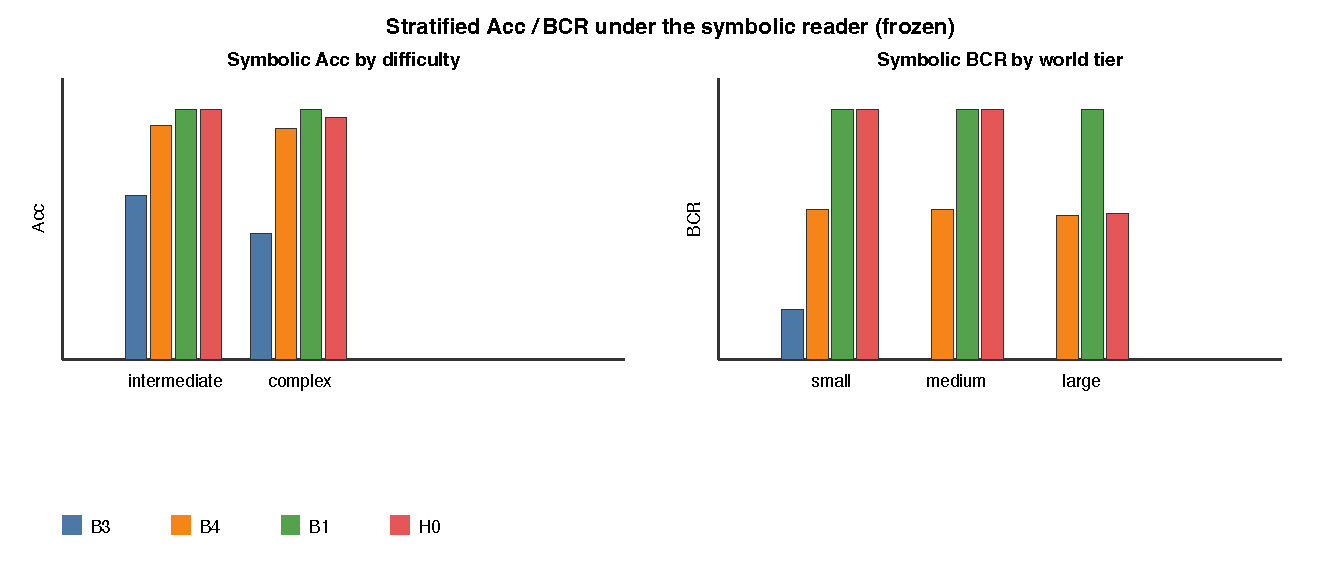
\includegraphics[width=0.95\linewidth]{figures/fig5-difficulty-tier.pdf}
\caption{Symbolic Acc by difficulty and BCR by world tier.}
\label{fig:difficulty}
\end{figure}

\begin{table}[t]
\centering
\caption{Constraint-family violation rates (headline systems).}
\label{tab:constraints}
\scriptsize
\begin{tabular}{lrrrr|rrr}
\toprule
& \multicolumn{4}{c|}{Symbolic} & \multicolumn{3}{c}{Qwen} \\
Family & B3 & B4 & B1 & H0 & B1/B3 & B4 & H0 \\
\midrule
uniqueness & 0.156 & 0.000 & 0.000 & 0.000 & 0.219 & 0.177 & 0.000 \\
temporal & 0.406 & 0.000 & 0.000 & 0.156 & 0.354 & 0.323 & 0.281 \\
transition & 0.375 & 0.120 & 0.000 & 0.000 & 1.000 & 1.000 & 1.000 \\
relational & 0.562 & 0.343 & 0.000 & 0.000 & 0.625 & 0.625 & 0.625 \\
provenance & 0.625 & 0.057 & 0.000 & 0.000 & 0.938 & 0.724 & 1.000 \\
multi\_hop & 0.344 & 0.124 & 0.000 & 0.000 & 0.406 & 0.406 & 0.406 \\
contradiction & 0.000 & 0.000 & 0.000 & 0.000 & 0.052 & 0.073 & 0.188 \\
\bottomrule
\end{tabular}
\end{table}

\begin{table}[t]
\centering
\caption{Query-family Acc under Qwen (H4; frozen; three-decimal display).}
\label{tab:queryfam}
\scriptsize
\begin{tabular}{lrrrr}
\toprule
Family & B1 & B3 & B4 & H0 \\
\midrule
current\_state & 0.010 & 0.010 & 0.083 & 0.542 \\
historical\_state & 0.162 & 0.162 & 0.089 & 0.547 \\
transition & 0.000 & 0.000 & 0.000 & 0.000 \\
multi\_hop & 0.000 & 0.000 & 0.052 & 0.000 \\
provenance & 0.188 & 0.167 & 0.417 & 0.000 \\
temporal\_order & 0.128 & 0.128 & 0.205 & 0.308 \\
contradiction & 0.083 & 0.083 & 0.167 & 0.000 \\
counterfactual & 0.000 & 0.000 & 0.000 & 0.000 \\
conflict\_validity & 0.462 & 0.462 & 0.462 & 0.000 \\
\bottomrule
\end{tabular}
\end{table}

\begin{table}[t]
\centering
\caption{\textbf{Frozen.} Symbolic H0 component ablations (reprinted from freeze CSV). Large Acc--BCR gaps under archive/temporal/graph removals.}
\label{tab:ablations}
\small
\begin{tabular}{lrrr}
\toprule
System & Acc & BCR & $\Gapq$ \\
\midrule
H0 unconstrained & 1.000 & 1.000 & 0.000 \\
H0 cap150 ret8 & 0.976 & 0.844 & 0.132 \\
H--archive & 0.876 & 0.375 & 0.501 \\
H--temporal-validity & 0.876 & 0.375 & 0.501 \\
H--graph & 0.938 & 0.594 & 0.344 \\
H--provenance & 1.000 & 1.000 & 0.000 \\
H--conflict & 0.800 & 0.812 & $-$0.012 \\
\bottomrule
\end{tabular}
\end{table}

\begin{table}[t]
\centering
\caption{\textbf{Labelled NEW.} Shortcut baselines (seed 100; 6 worlds/tier; symbolic scoring). Family-majority uses oracle gold marginals by query family.}
\label{tab:shortcuts}
\small
\begin{tabular}{lrrr}
\toprule
Baseline & Acc & BCR & $\Gapq$ \\
\midrule
Empty answers & 0.000 & 0.000 & 0.000 \\
Family-majority (gold marginals) & 0.352 & 0.000 & 0.352 \\
Family-shuffle of gold answers & 0.280 & 0.000 & 0.280 \\
Gold oracle & 1.000 & 1.000 & 0.000 \\
\bottomrule
\end{tabular}
\end{table}

\begin{table}[t]
\centering
\caption{\textbf{Labelled NEW.} Seed sweep summary (symbolic B3/B4 $k{=}8$; 6 worlds/tier; seeds 100--105). B3 identical across seeds (limited diversity).}
\label{tab:seeds}
\small
\begin{tabular}{lrrr}
\toprule
System & Acc range & BCR & $\Gapq$ range \\
\midrule
B3 recency-$k8$ & 0.567--0.567 & 0.0625 & 0.504--0.504 \\
B4 BM25-$k8$ & 0.929--0.932 & 0.5938 & 0.335--0.338 \\
\bottomrule
\end{tabular}
\end{table}

\begin{table}[t]
\centering
\caption{\textbf{Labelled NEW.} Generator controls (symbolic). Density: 8 medium worlds, seed base 200. Distractors: seed 100, wpt$=$6.}
\label{tab:density}
\small
\begin{tabular}{llrrr}
\toprule
Control & Setting & System & Acc & BCR \\
\midrule
Relation density & 0.0 / 1.0 & B4 & 0.917 / 0.909 & 0.600 / 0.600 \\
Relation density & 0.0 / 1.0 & B3 & 0.545 / 0.545 & 0.000 / 0.000 \\
Distractors & on / off & B4 & 0.932 / 0.932 & 0.594 / 0.594 \\
Distractors & on / off & B3 & 0.567 / 0.567 & 0.062 / 0.062 \\
\bottomrule
\end{tabular}
\end{table}

\begin{table}[t]
\centering
\caption{Evaluation coverage and hard limits.}
\label{tab:coverage}
\begin{tabular}{ll}
\toprule
Dimension & Coverage \\
\midrule
Paper shape & Benchmark + evaluation methodology \\
Symbolic reader & Full scaled (102 / 1{,}088 / 7{,}140) \\
LLM reader & Qwen2.5-3B-Instruct-4bit; H4 subset only \\
Stronger LLM readers & Not completed in this submission environment \\
Architecture superiority & Unsupported under Qwen (all BCR~$=$~0) \\
Ecological validity & Not claimed (synthetic worlds) \\
Primary consistency metric & BCR (strict); CSR complementary \\
Labelled robustness & Seeds/density/distractors/shortcuts (separate tables) \\
\bottomrule
\end{tabular}
\end{table}
